% Created 2020-05-22 Fri 11:41
% Intended LaTeX compiler: pdflatex
\documentclass[presentation]{beamer}
\usepackage[utf8]{inputenc}
\usepackage[T1]{fontenc}
\usepackage{graphicx}
\usepackage{grffile}
\usepackage{longtable}
\usepackage{wrapfig}
\usepackage{rotating}
\usepackage[normalem]{ulem}
\usepackage{amsmath}
\usepackage{textcomp}
\usepackage{amssymb}
\usepackage{capt-of}
\usepackage{hyperref}
\usetheme{UoB}
\author{Mark Blyth}
\date{\textit{[2020-05-25 Mon]}}
\title{Spring project summary}
\hypersetup{
 pdfauthor={Mark Blyth},
 pdftitle={Spring project summary},
 pdfkeywords={},
 pdfsubject={},
 pdfcreator={Emacs 26.3 (Org mode 9.1.9)}, 
 pdflang={English}}
\begin{document}

\maketitle

\section{Previous}
\label{sec:orgf89715d}
\begin{frame}[label={sec:orga023713}]{Last meeting}
Discussion about single-cell and multi-cell approaches
\vfill
Single-cell: 
\begin{itemize}[<+->]
\item Strong literature precedent for what to expect
\item Lots of accepted models to test \emph{in-silico}
\item Easy-to-spot bifurcations
\begin{itemize}
\item Hopf, fold both easily detectable with CBC
\end{itemize}
\item Reuse Bath single-cell microfluidics device
\end{itemize}
\end{frame}


\begin{frame}[label={sec:orgbf79652}]{Last meeting}
Discussion about single-cell and multi-cell approaches
\vfill
Multi-cell: 
\begin{itemize}[<+->]
\item Assume there's an arbitrarily large number of cells
\begin{itemize}
\item Neural continuum fields (limited descriptive ability)
\item Spatially extended cubic Lienard system
\end{itemize}
\item Search experimentally and numerically for PDE bifurcations
\begin{itemize}
\item Not an area I know much about (yet\ldots{})
\end{itemize}
\item Can build on work by Krasi's Munich collaborators
\item Or could reuse Bath microfluidic device
\begin{itemize}
\item Would require minor alterations to increase spatial resolution
\end{itemize}
\end{itemize}
\end{frame}


\begin{frame}[label={sec:orgcf8136c}]{Single- vs multi-cell}
Deciding factors:

\vfill

\begin{itemize}
\item No lab access for the forseeable future
\begin{itemize}
\item Work can be guided less by experiments
\end{itemize}
\item Single-cell easier than multi-cell
\begin{itemize}
\item I know enough about single-cell CBC to start working on it
\end{itemize}
\end{itemize}

\vfill

Conclusion: work on single-cell case
\end{frame}


\section{Current}
\label{sec:org6d77b43}
\begin{frame}[label={sec:org17690ff}]{Current goals}
\begin{itemize}
\item Single-cell \emph{in-silico} CBC
\item Tutorial-review paper for numerical continuation
\end{itemize}
\end{frame}

\begin{frame}[label={sec:org67b7d3c}]{Challenges of \emph{in-silico} CBC}
Data aren't ideal to work with:
\vfill
\begin{itemize}
\item Real signals are noise-corrupted
\begin{itemize}
\item Difficult to filter off, since spikes contain lots of high-frequency components
\item Hard to run continuation on stochastic and noisy signals
\item Current work
\end{itemize}
\end{itemize}
\vfill
\begin{itemize}
\item Neurons are fast-spiking
\begin{itemize}
\item Fourier discretisation won't work
\item Discretisations need to be very high-dimensional, making Jacobian very slow to find
\item Next work
\end{itemize}
\end{itemize}

\vfill
\end{frame}

\begin{frame}[label={sec:org90d13d2}]{Issue 1: noise corruption}
Instead of running continuation on noisy signal measurements, let's run it on a surrogate data source

\begin{center}
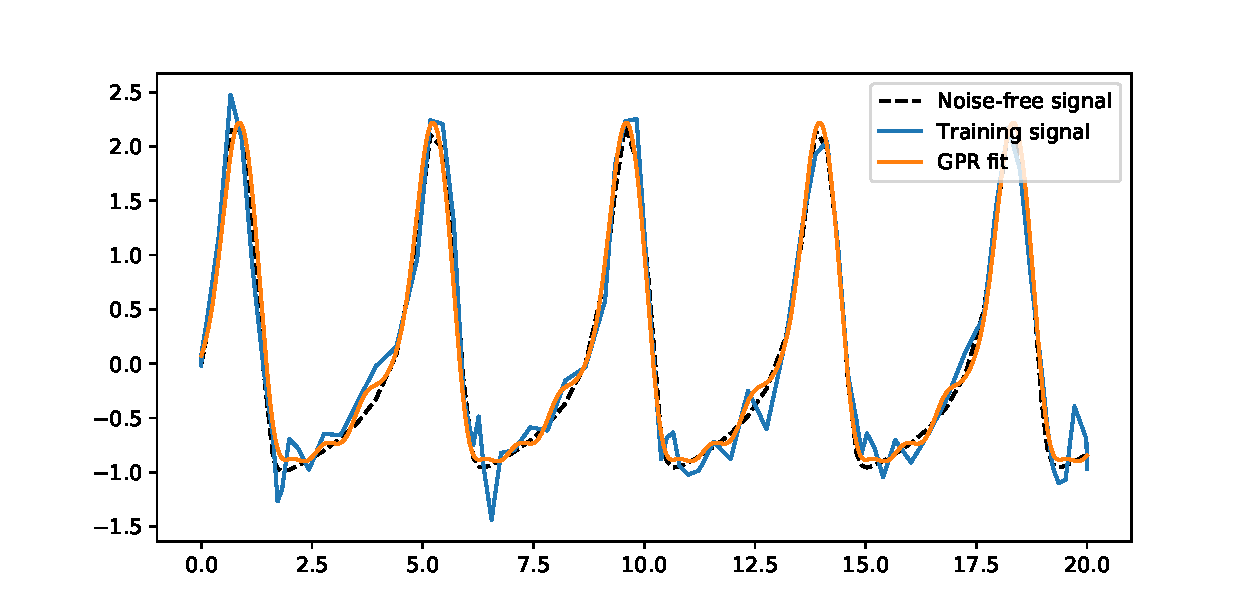
\includegraphics[width=.9\textwidth]{./GPR_demo.pdf}
\end{center}
\end{frame}

\begin{frame}[label={sec:orgf7e66b6}]{Surrogate models}
Surrogate models don't always work well!

\begin{center}
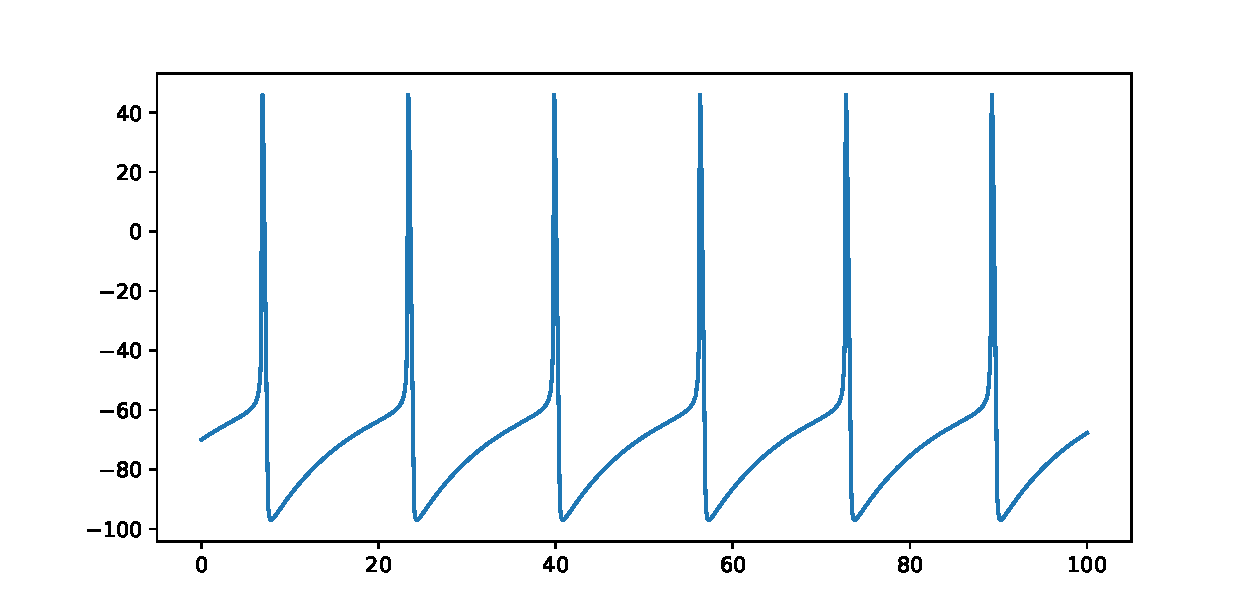
\includegraphics[width=.9\textwidth]{./HHraw.pdf}
\end{center}
\end{frame}

\begin{frame}[label={sec:orgd250d0d}]{Surrogate models}
Surrogate models don't always work well!

\begin{center}
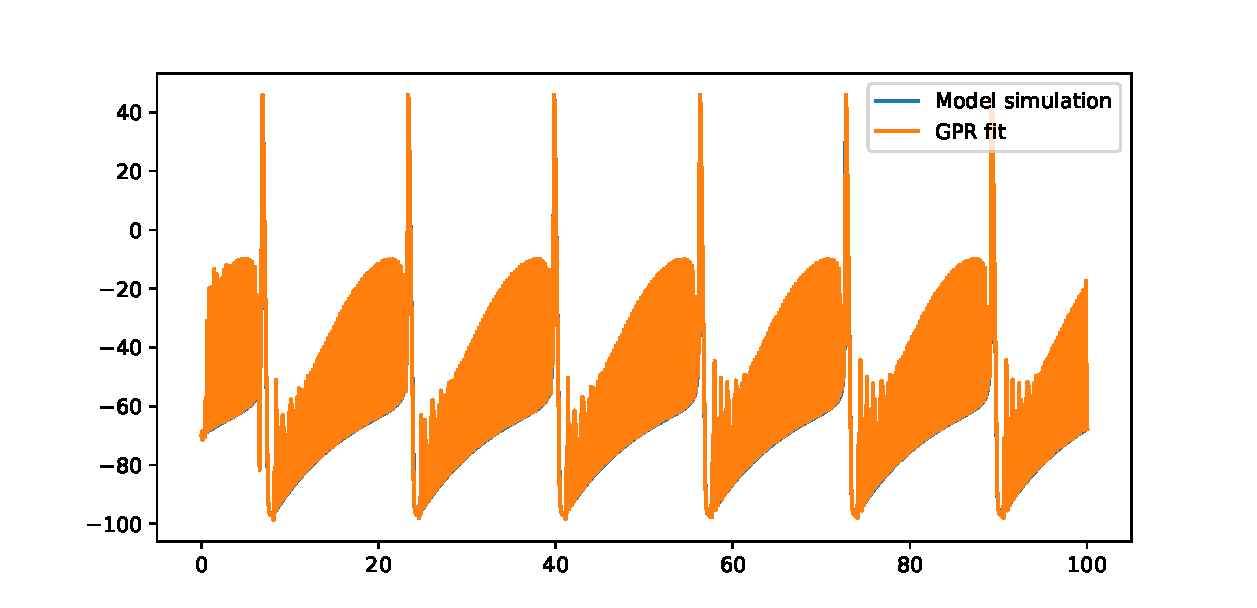
\includegraphics[width=.9\textwidth]{./HH.pdf}
\end{center}
\end{frame}


\begin{frame}[label={sec:orgabca2d7}]{Machine learning for dynamical systems}
\begin{itemize}
\item Current approach: Gaussian process regression
\begin{itemize}
\item Predict new points as an intelligently weighted sum of example points
\end{itemize}
\item Bayesian kernel method
\begin{itemize}
\item Kernel specifies a distribution over basis functions
\item Good kernel choice = good data fit
\end{itemize}
\item Most kernels are stationary, and can't handle the spiking behaviours of neurons
\end{itemize}

\vfill

Current goal: find an ML approach to fitting a surrogate model
\end{frame}


\section{Next}
\label{sec:orgd022894}

\begin{frame}[label={sec:orgd519b16}]{Next questions}
\begin{itemize}
\item Predictor-corrector design
\item Stochastic models
\end{itemize}
\end{frame}

\begin{frame}[label={sec:org4e4a4ab}]{Continuation issues}
\begin{itemize}
\item Discretisation is required to make predictor-corrector methods work
\item It has issues for fast-spiking data
\begin{itemize}
\item Slow to find a Jacobian
\item High noise-sensitivity
\end{itemize}
\item Discretisation-free predictor-correctors might overcome these
\end{itemize}
\end{frame}

\begin{frame}[label={sec:orgb927845}]{Alternative continuation approach}
Predictor-corrector design:
\vfill
\begin{itemize}
\item We could try discretisation-free predictor steps, using a surrogate model
\begin{itemize}
\item Let \(f_i(t)\) be the surrogate model for system behaviours at parameter \(\lambda_i\)
\item Given periodic orbits \(f_{i-1},~f_i\), predict \(f_{i+1} = f_i + h \big[f_i - f_{i-1}\big]\)
\end{itemize}
\item Corrector step would be harder
\end{itemize}
\end{frame}

\begin{frame}[label={sec:orga1223d4}]{An idea for discretisation-free correction}
Main goal of CBC: find \(x^*(t)\) such that \(\forall t, u(x,x^*)=0\).

\vfill
Alternative formulation:
\begin{itemize}[<+->]
\item Let \(S[x^*] = \int_0^T u^2(x,x^*) \mathrm{d}t\) measure control invasiveness
\item \(S: \mathcal{H} \to \mathbb{R}\) is a functional on control actions \(x^*\)
\item CBC becomes a calculus of variations problem; find \(x^*(t)\) that minimises \(S\)
\item \(S=0\) if and only if \(x^*(t)\) is an invariant set of the open-loop system
\end{itemize}

\vfill
\end{frame}
\begin{frame}[label={sec:org540d2f5}]{Calculus of variations}
Alternative formulation: find \(x^*(t)\) that minimises \(S[x^*]\)

\vfill

\begin{itemize}
\item Calculus of variations provides a framework for finding minimising functions
\item Might be possible to define an iteration scheme on functions, rather than discretisations
\end{itemize}

\vfill
Calculus of variations
\begin{itemize}
\item Well-studied in control theory; lots of precedent to build on
\item Shifts the noninvasiveness requirement away from the continuation scheme, and onto the controller
\end{itemize}
\end{frame}

\begin{frame}[label={sec:org8a12d41}]{Variational noninvasiveness}
Ideally, corrector would find some iteration sequence \(f_1,~f_2,~\dots\), such that \(S[f_i] > S[f_{i-1}]\)
\begin{itemize}
\item Then we've found a function-space iteration scheme to reach noninvasive control
\item Works on functions at every step, so we avoid the issues of discretisation
\end{itemize}
\vfill
Might be a dead-end.
\end{frame}

\begin{frame}[label={sec:org3f46807}]{Variational noninvasiveness}
Overall idea:
\begin{itemize}
\item Set up CBC as a calculus of variations problem
\item Reach noninvasiveness by minimising functional \(S\)
\item Find a numerical method to do this though iterations on control target \(x^*(t)\)
\item Use the variational equations to reformulate Newton iterations onto functions, rather than vectors
\begin{itemize}
\item Main question: is this even possible?
\end{itemize}
\end{itemize}
\end{frame}

\begin{frame}[label={sec:orge1f8045}]{Stochastic models}
Real neurons are stochastic
\begin{itemize}
\item Stochasticity introduces new challenges
\begin{itemize}
\item Coherence and stochastic resonance
\item Random attractors
\item Stochastic calculus
\end{itemize}
\item Current work: CBC on noise-corrupted simulations
\item Next work: CBC on true stochastic models
\end{itemize}

\vfill
\end{frame}


\begin{frame}[label={sec:org3fe9893}]{Goals}
Actions:
\begin{itemize}
\item Find a surrogate modelling method for neural data
\item Attempt a discretisation-free corrector?
\item Run CBC on deterministic models, then stochastic
\end{itemize}

\vfill

Results:
\begin{itemize}
\item Write up surrogate modelling into a conference abstract \emph{[July]}
\begin{itemize}
\item Maybe a conference paper \emph{[September]}
\end{itemize}
\item Use surrogate modelling for an \emph{in-silico} CBC paper \emph{[next year?]}
\end{itemize}
\end{frame}
\end{document}
